En este anexo se presentan los planos de despiece y ensamble correspondientes a las principales piezas diseñadas para la mesa de pruebas de motores. Como se mencionó en el Capítulo~\ref{ch:CH05}, algunas de estas piezas deben personalizarse en función de la geometría del motor a ensayar, ya que cualquier variación en sus dimensiones impacta directamente en el diseño del soporte y, en consecuencia, en el acople del imán coaxial al sensor de efecto \textit{hall}. Esto se debe a que el acople debe fijarse al eje mediante un prisionero, cuyo diámetro o forma puede variar según el motor seleccionado. Del mismo modo, el soporte del sensor debe ajustarse de acuerdo con la altura del eje, con el fin de garantizar la mayor coaxialidad posible entre el imán y el elemento sensor.


\begin{landscape}
\label{plano base}
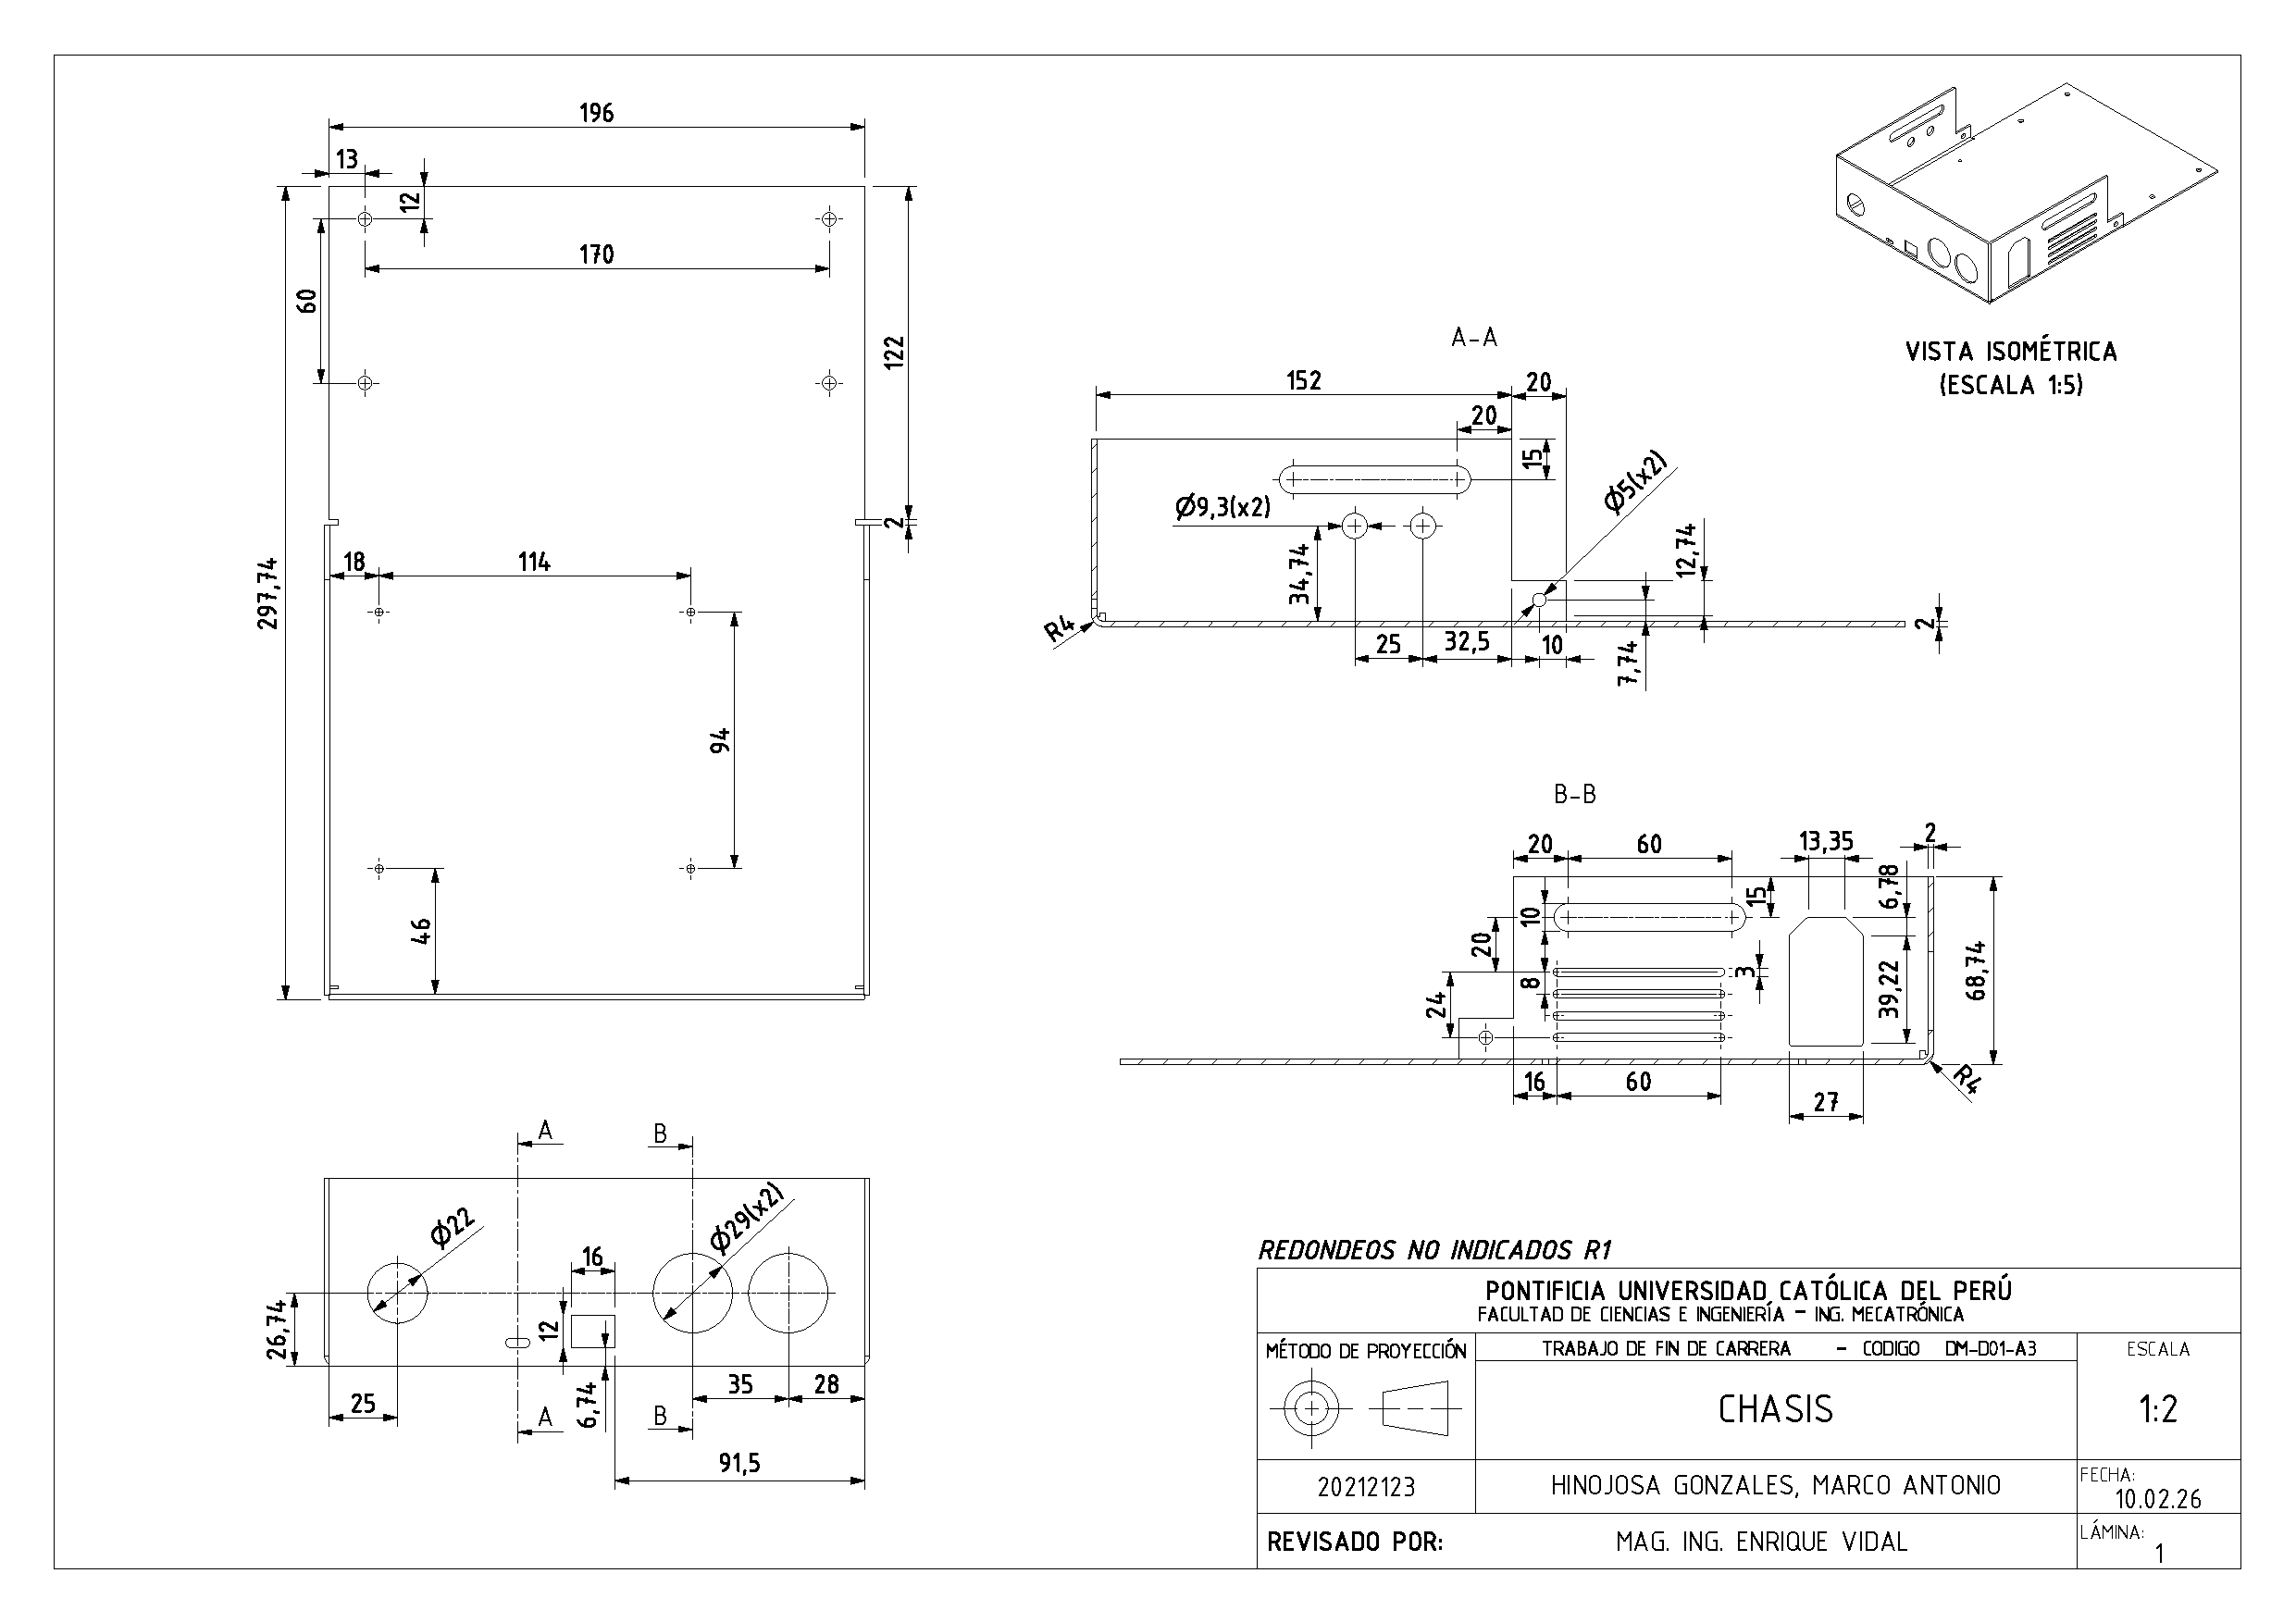
\includepdf[pages=1, landscape=true, fitpaper=true]{ANNEX/Fig/AS/CHASIS.pdf}
\end{landscape}

% --- PDF 2 en horizontal ---
\begin{landscape}
\label{plano ensamble}

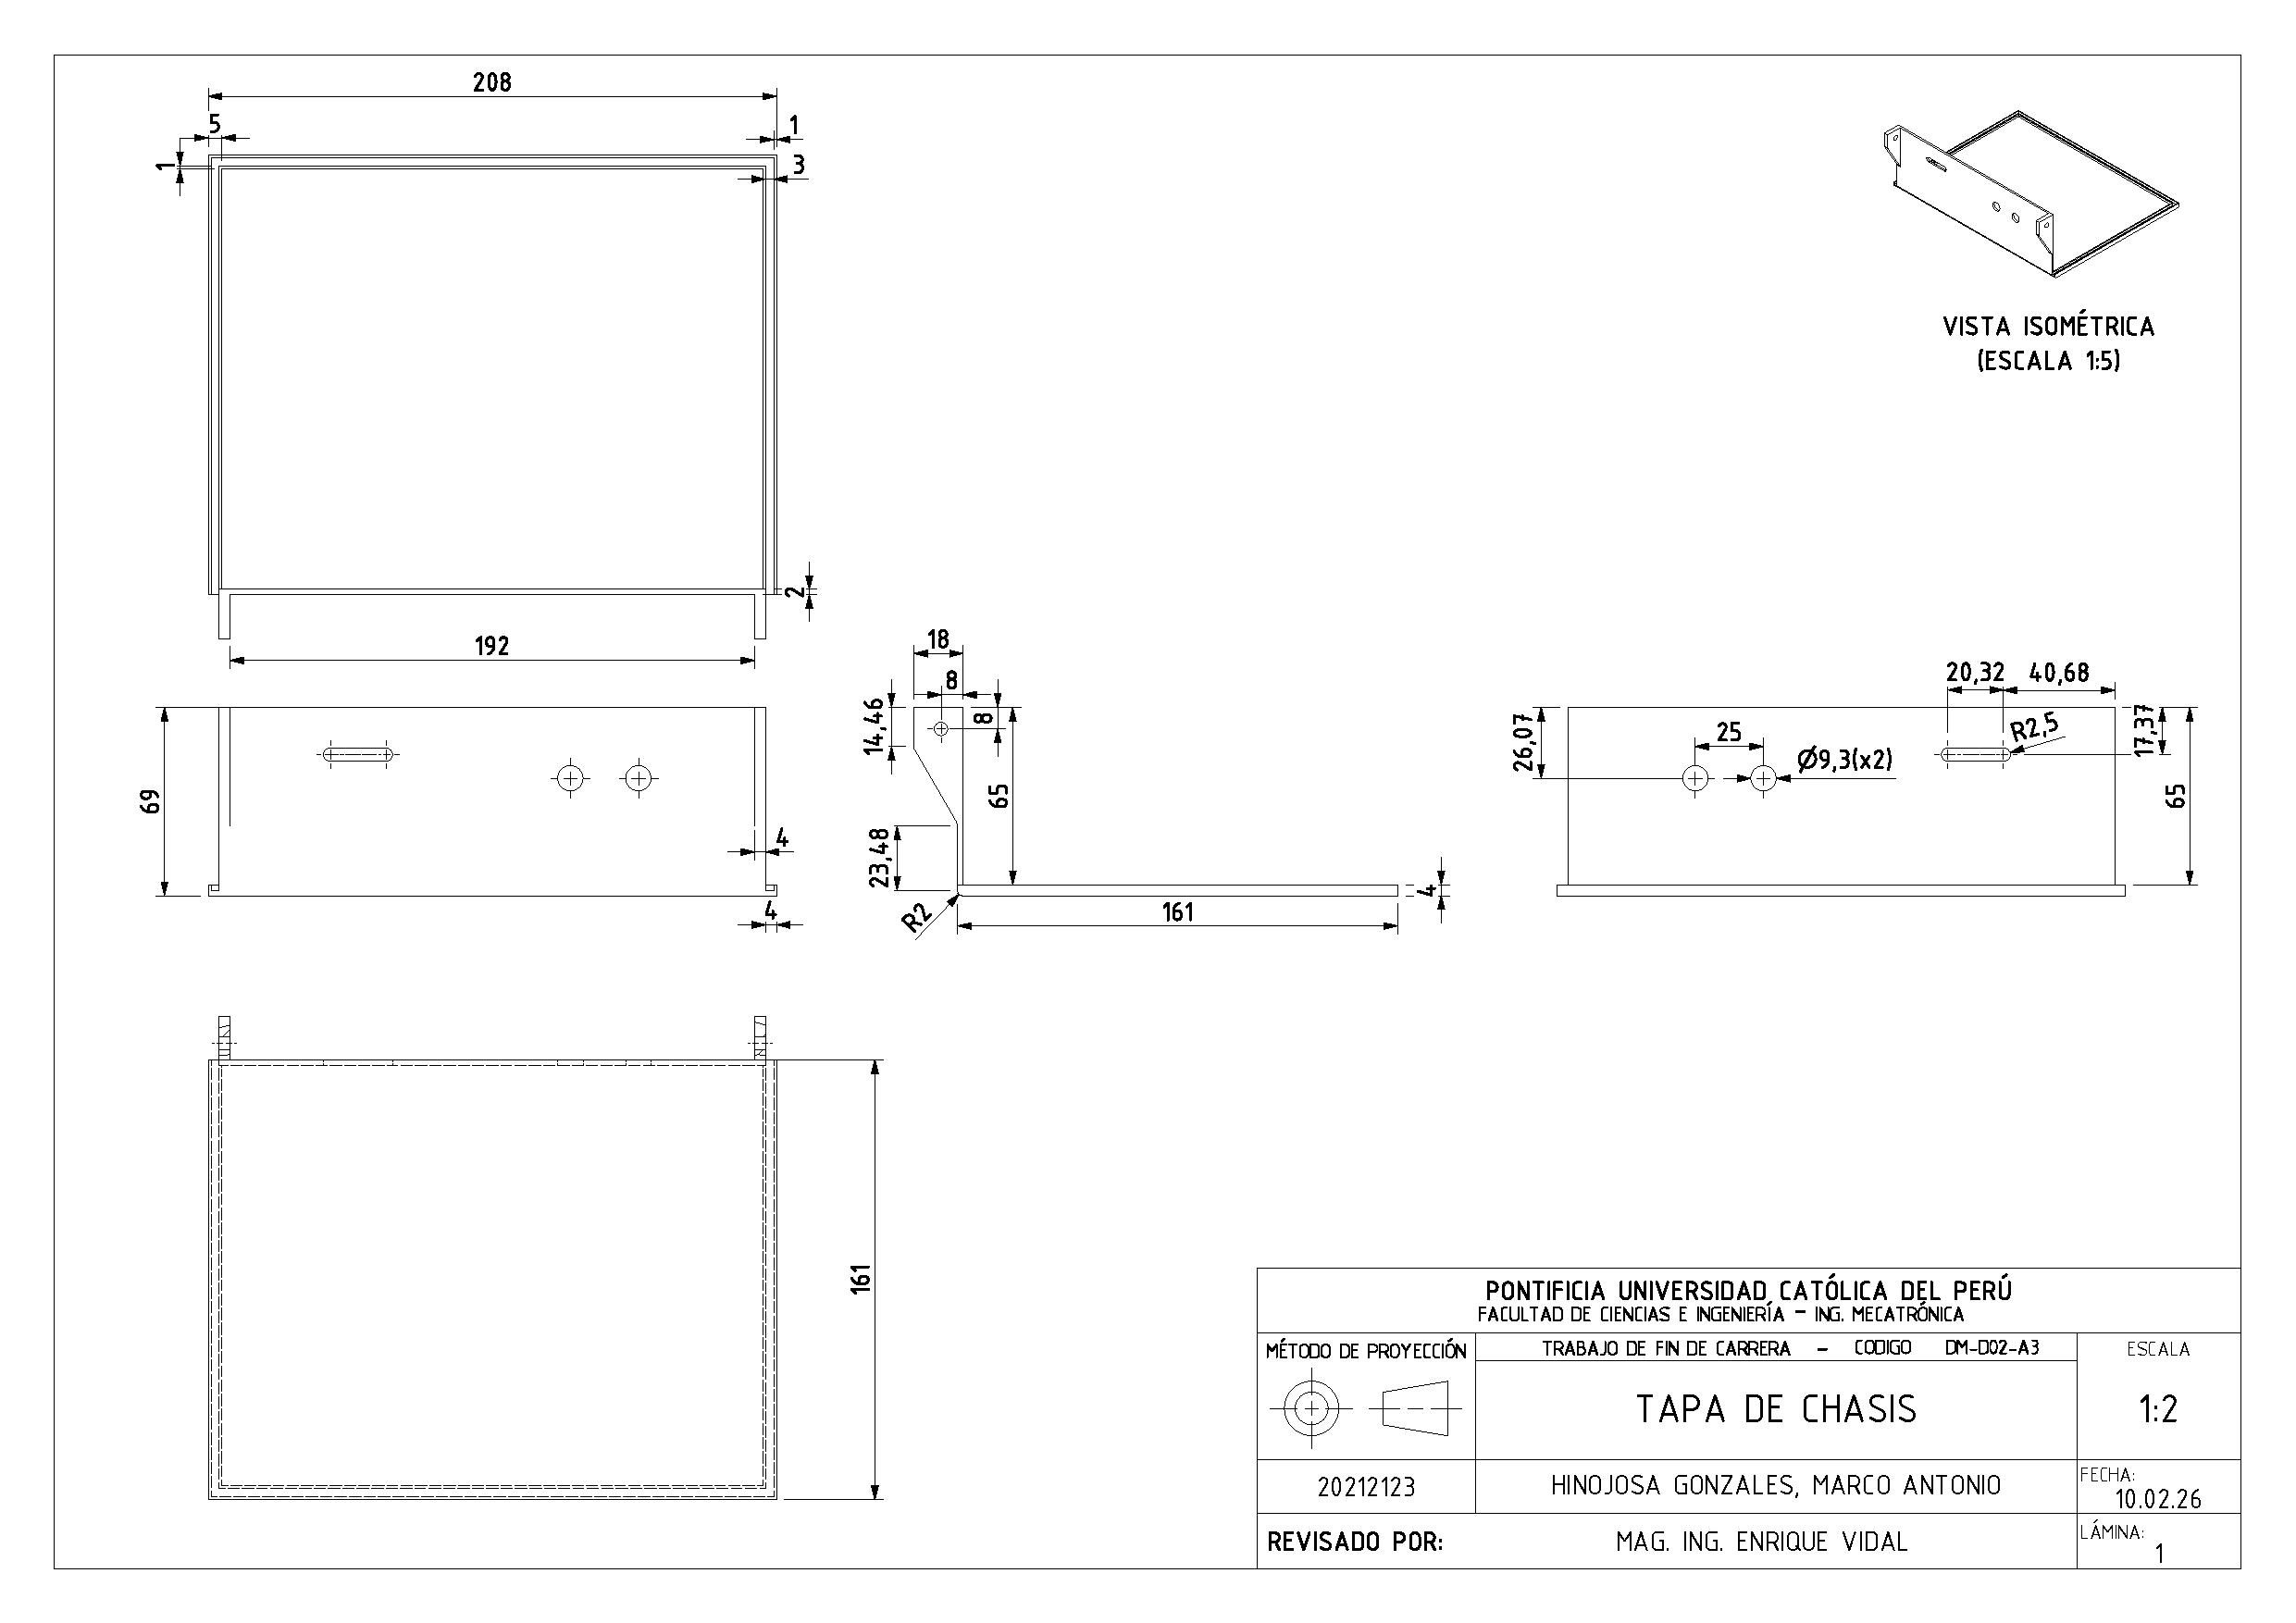
\includepdf[pages=1, landscape=true, fitpaper=true]{ANNEX/Fig/AS/TAPA_CHASIS.pdf}
\end{landscape}

% --- PDF 3 en horizontal ---
\begin{landscape}
\label{plano base superior}

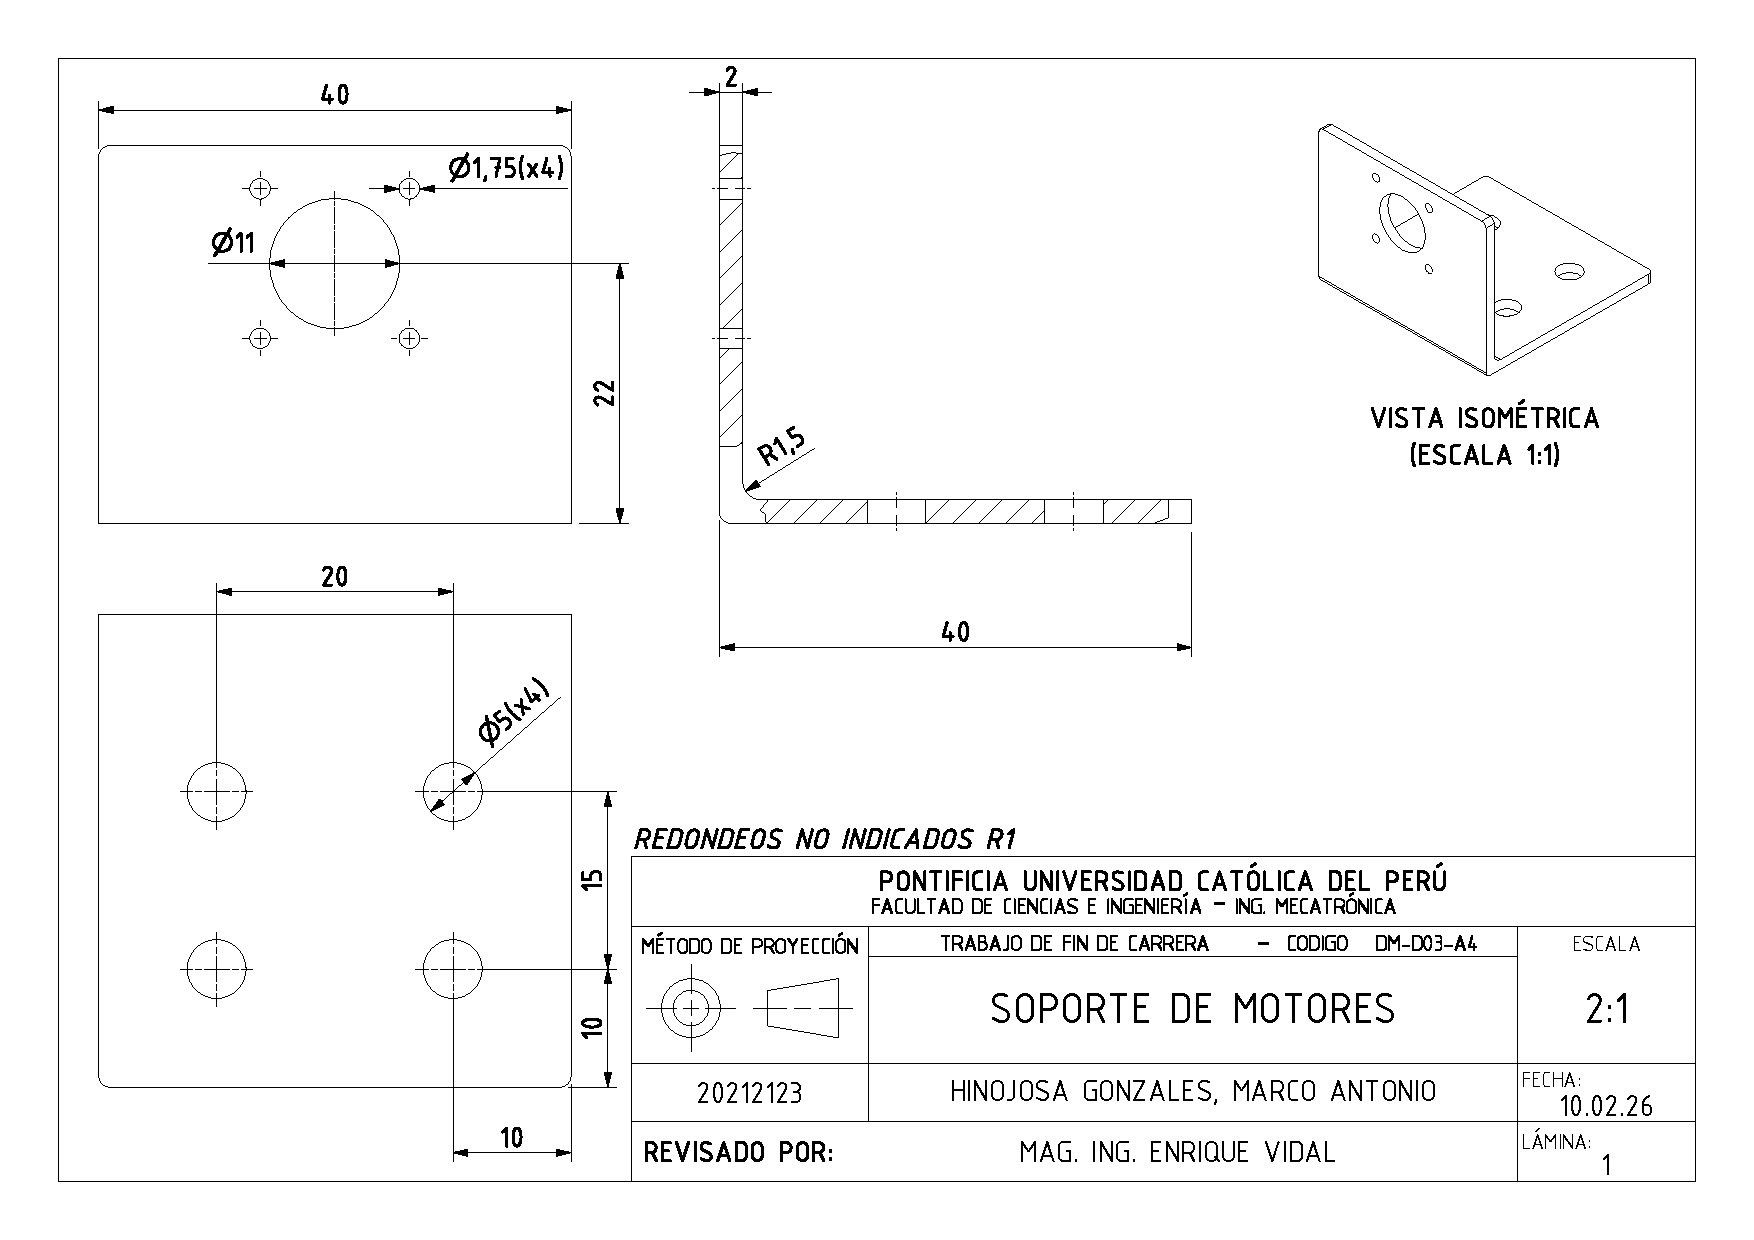
\includepdf[pages=1, landscape=true, fitpaper=true]{ANNEX/Fig/AS/BRACKET_MOTOR.pdf}
\end{landscape}

% --- PDF 4 en horizontal ---
\begin{landscape}
\label{plano ensamble}

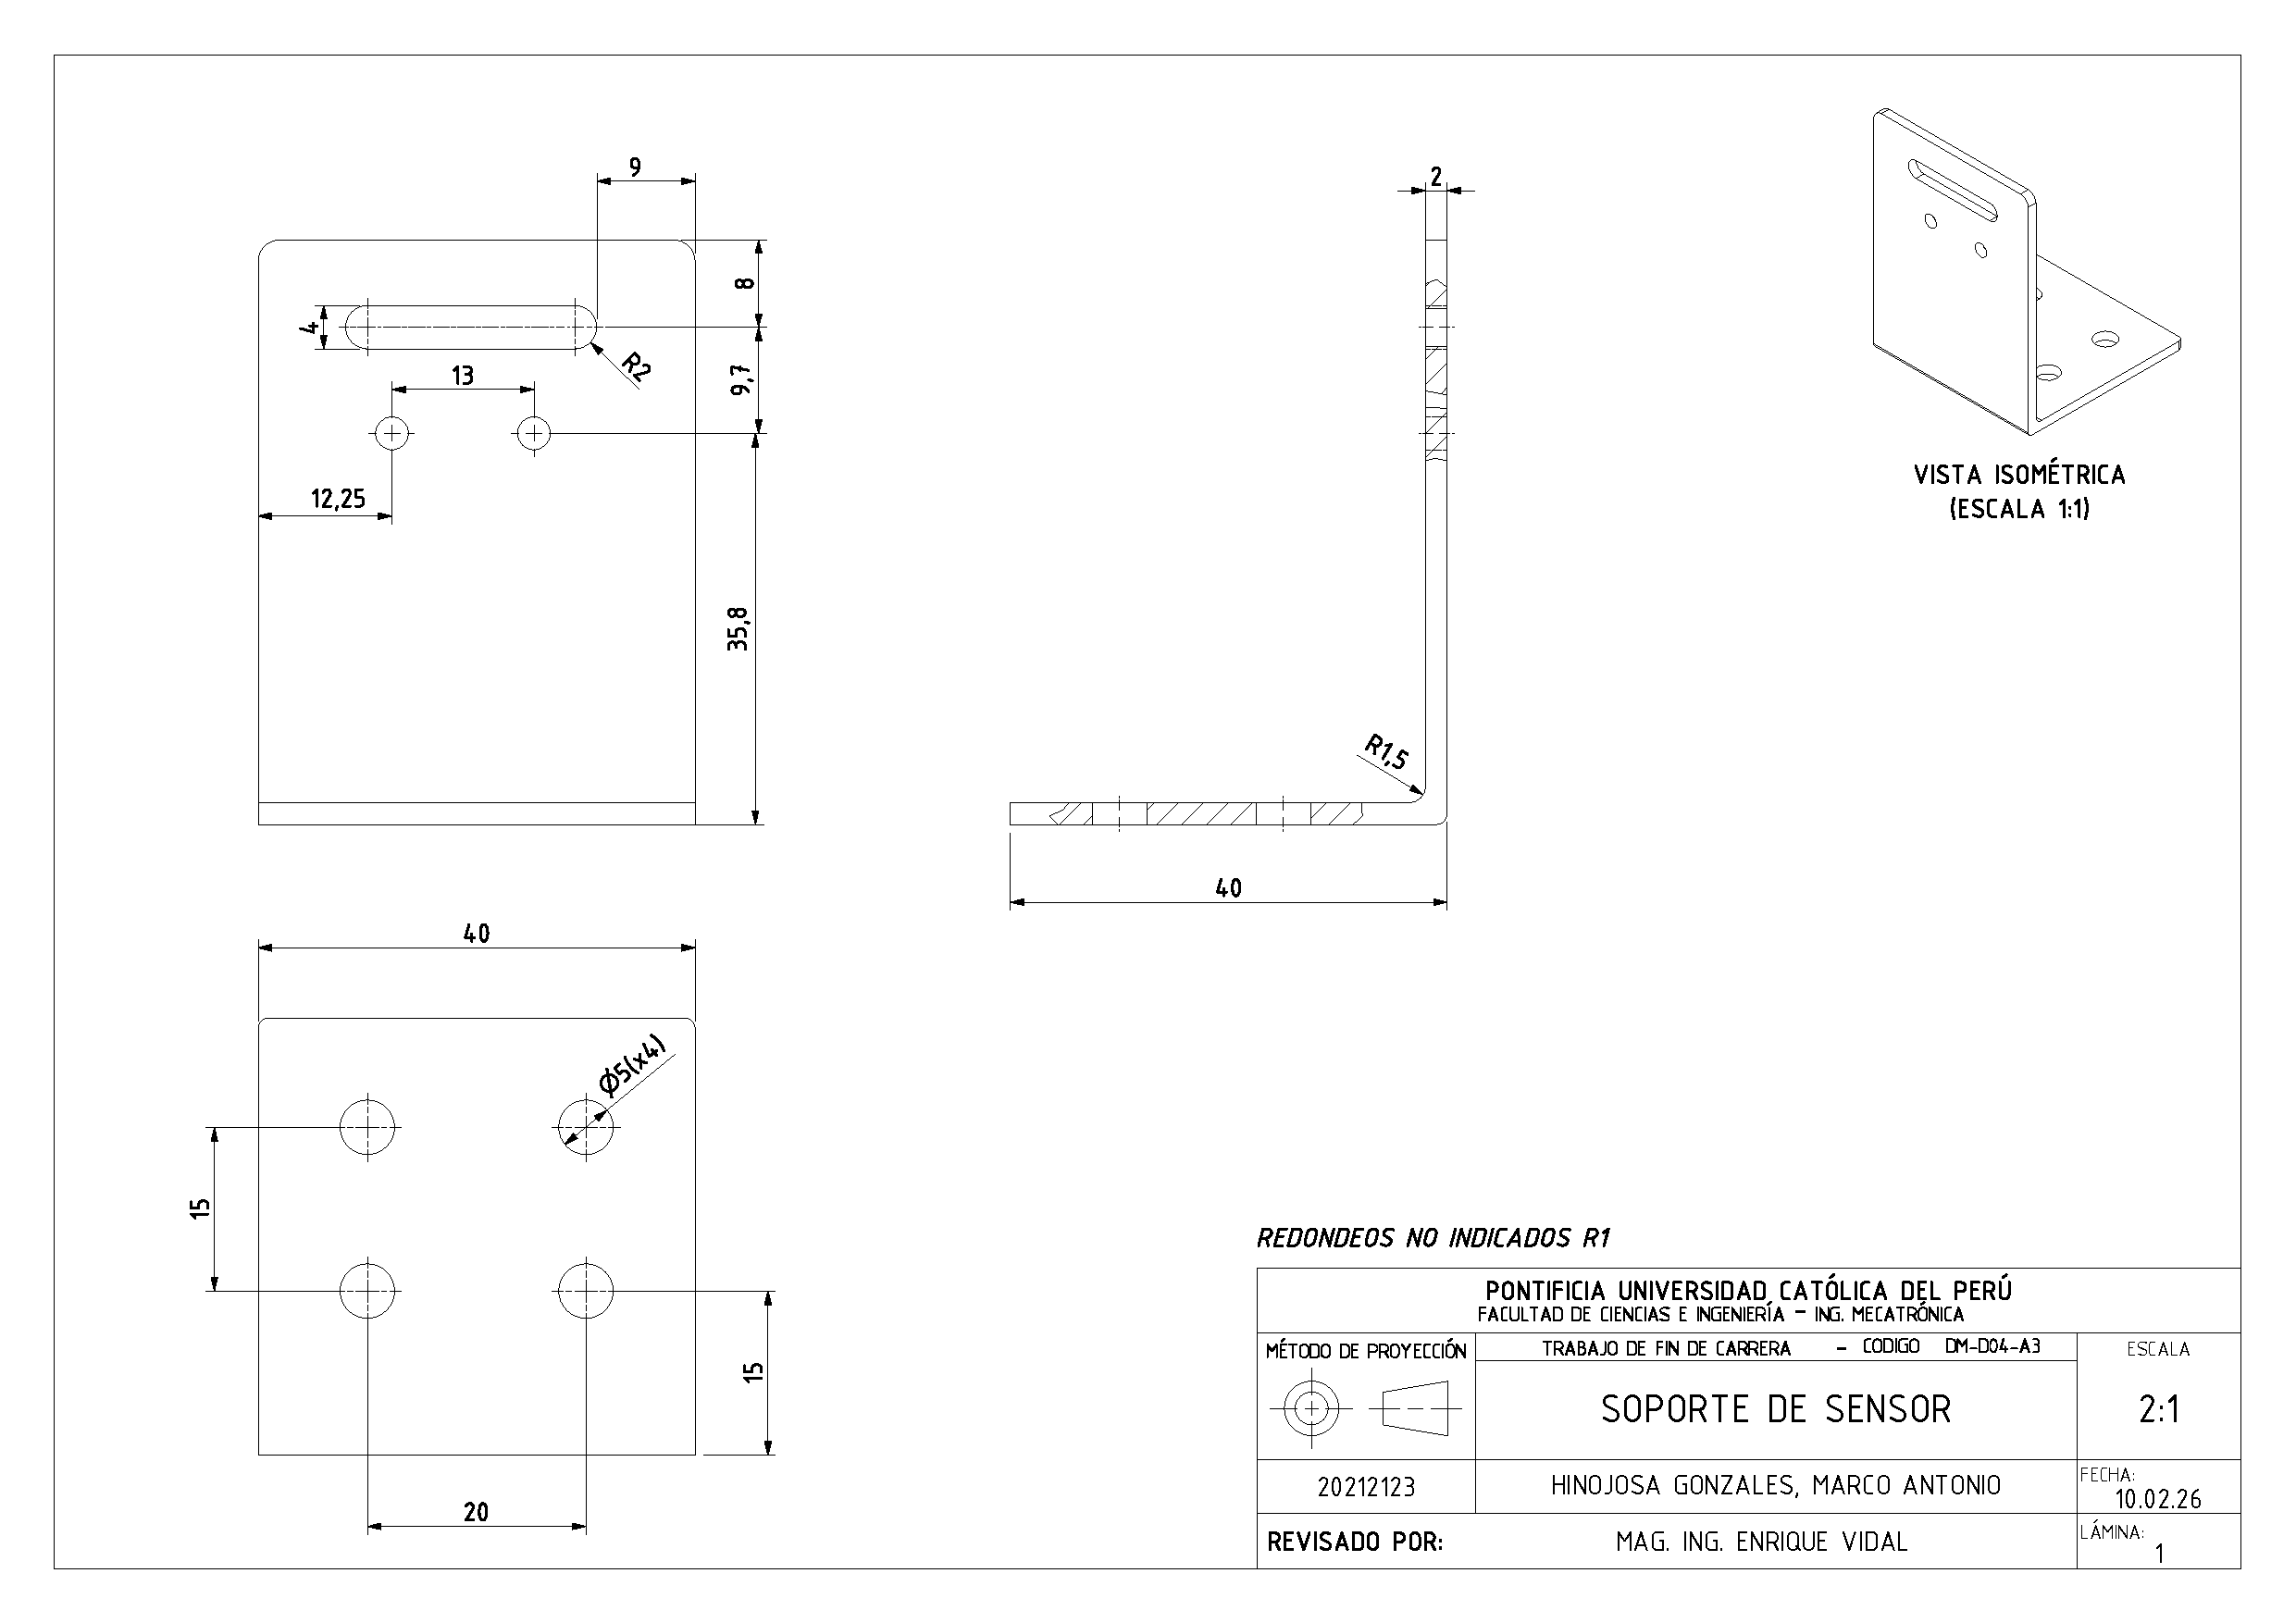
\includepdf[pages=1, landscape=true, fitpaper=true]{ANNEX/Fig/AS/BRACKET_SENSOR.pdf}
\end{landscape}

% --- PDF 5 en horizontal ---
\begin{landscape}
\label{plano ensamble}

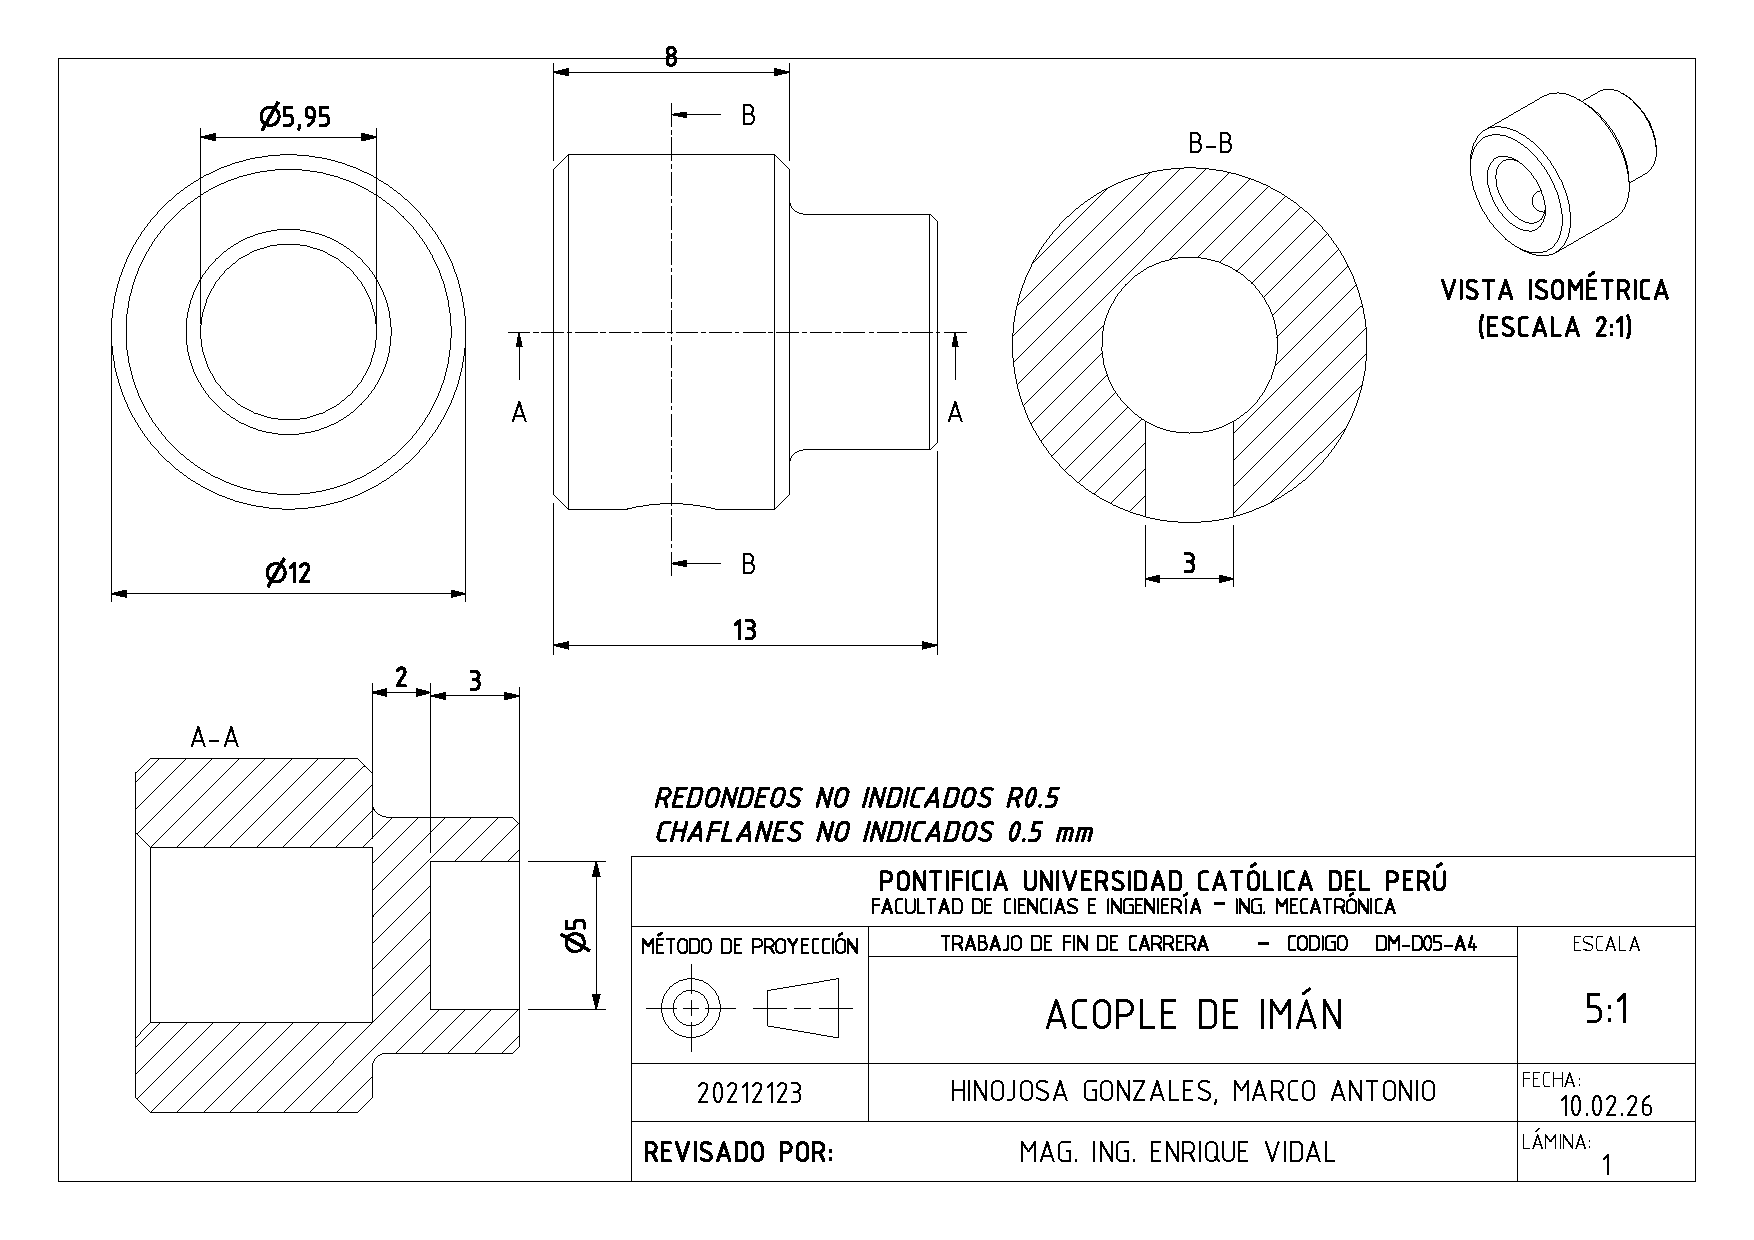
\includepdf[pages=1, landscape=true, fitpaper=true]{ANNEX/Fig/AS/Acople_IMAN-1.pdf}
\end{landscape}

% --- PDF 6 en horizontal ---
\begin{landscape}
\label{plano ensamble}

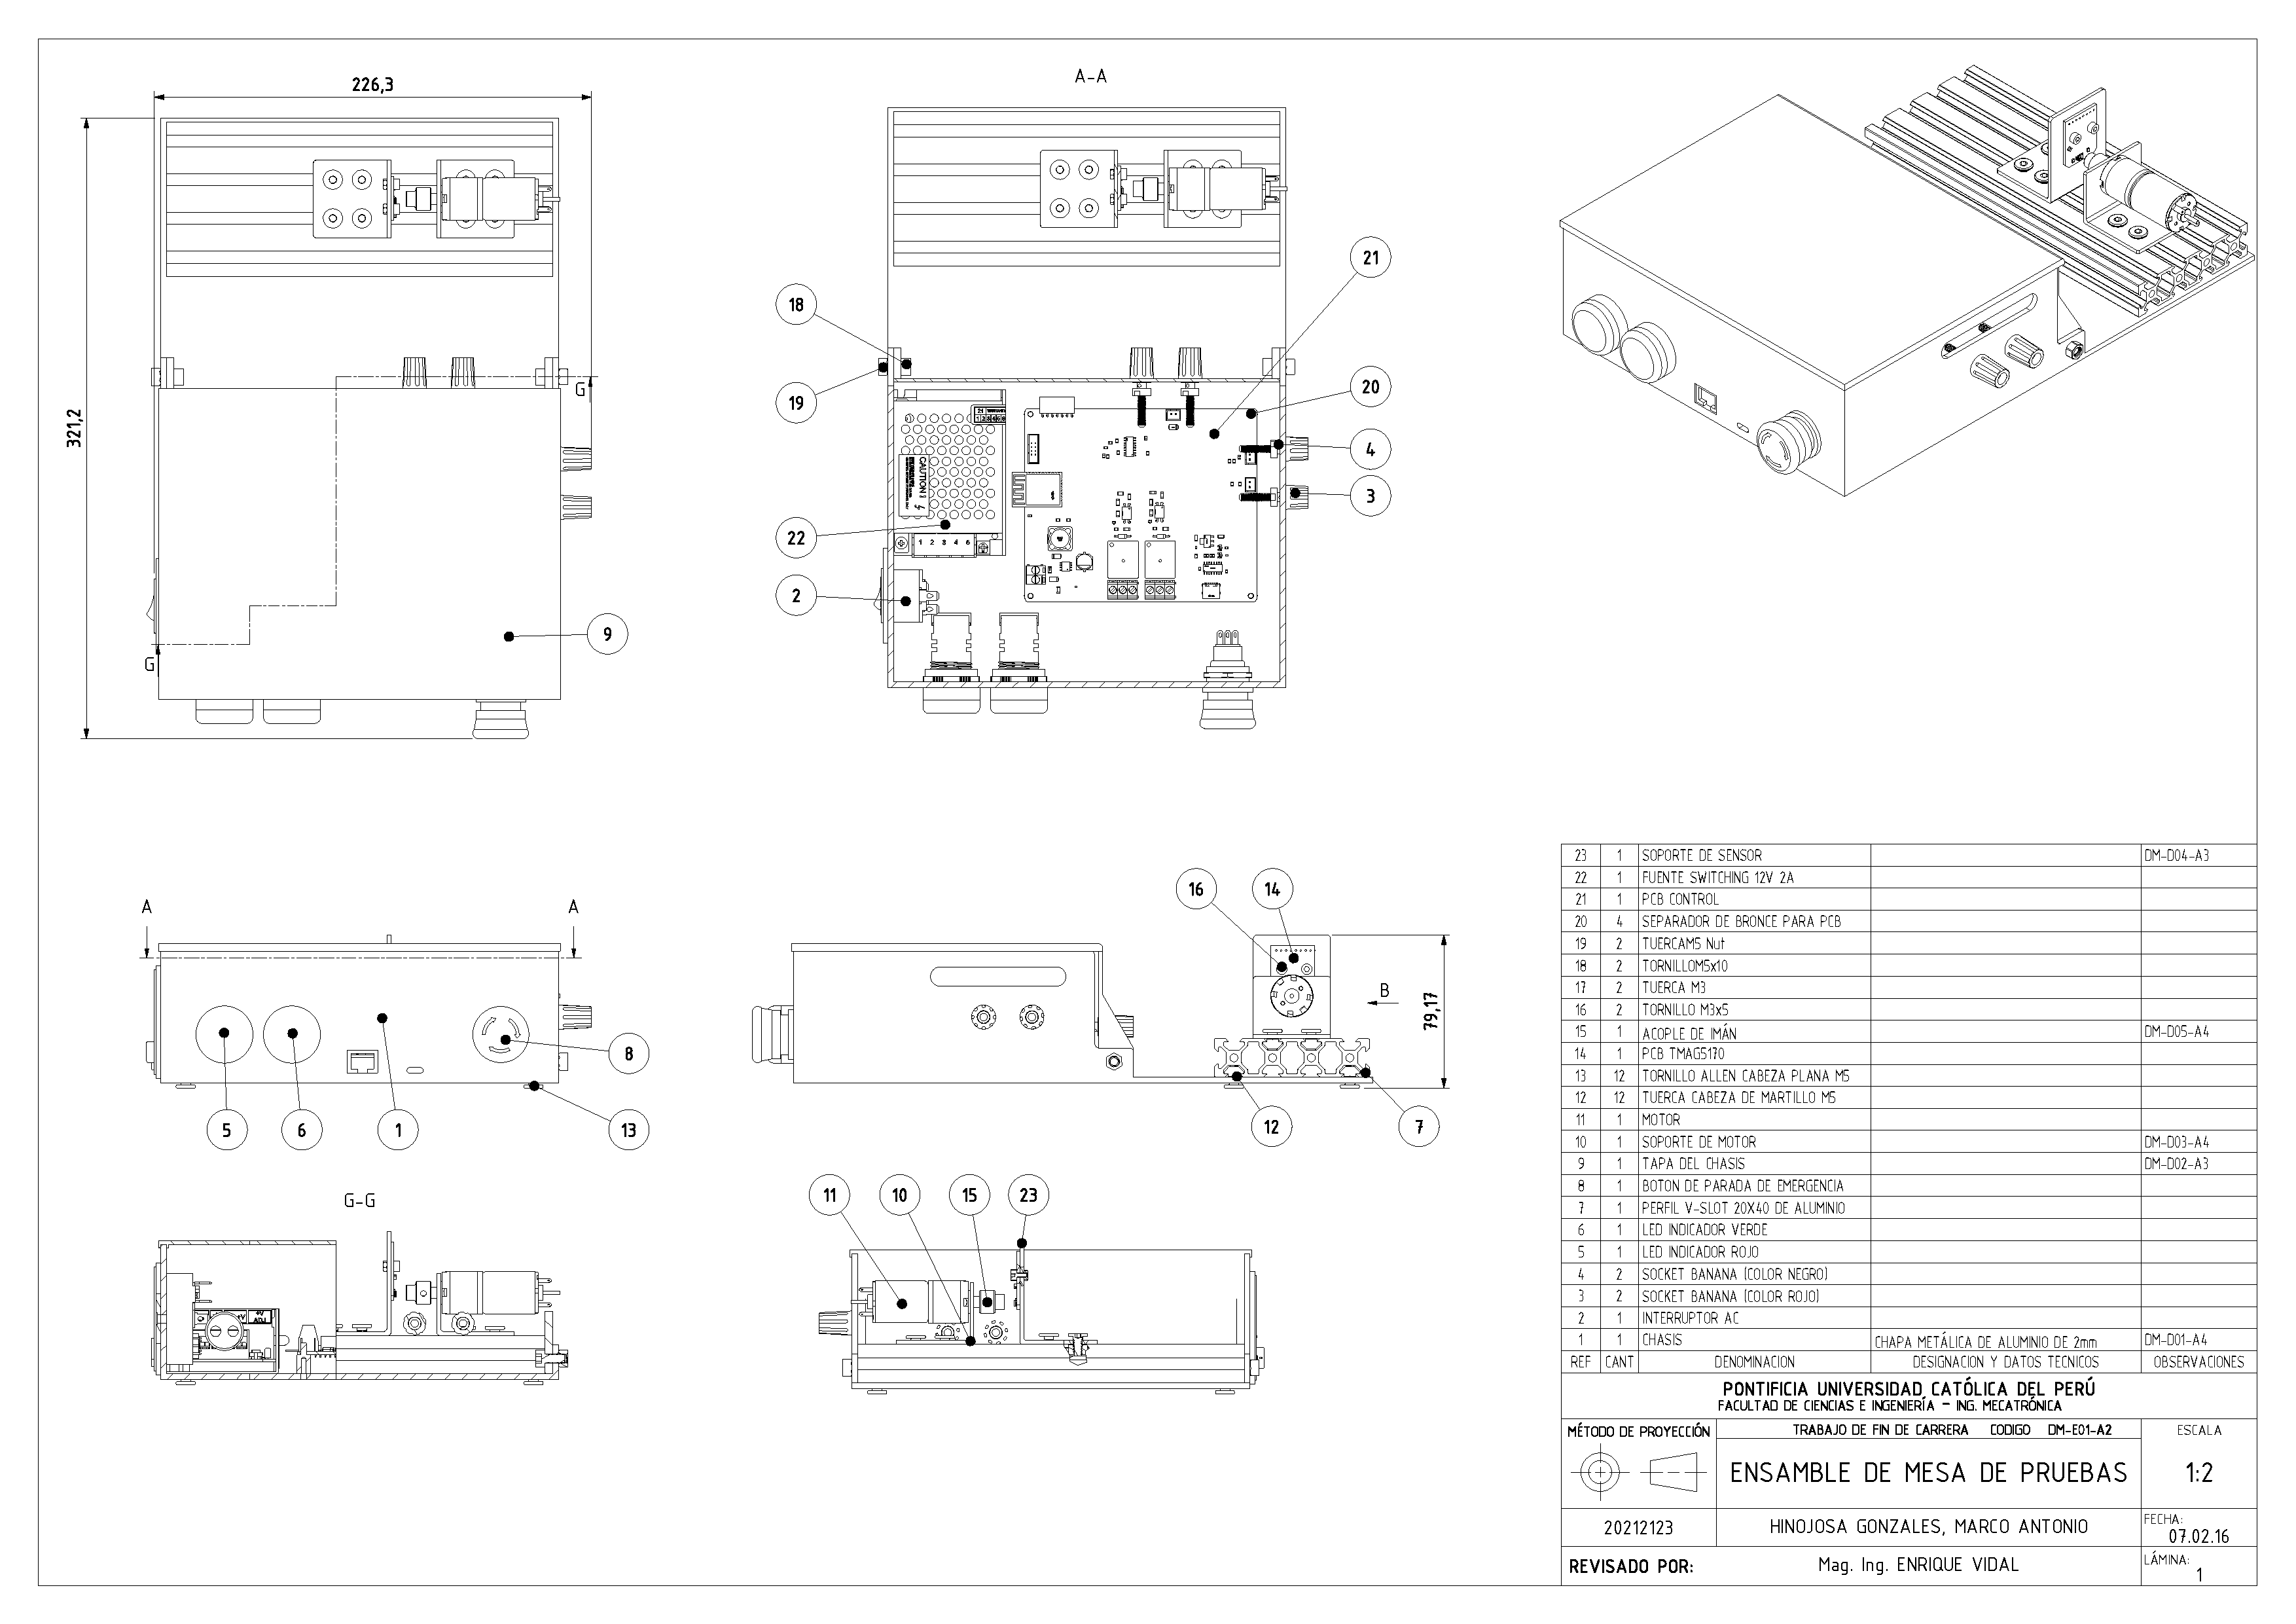
\includepdf[pages=1, landscape=true, fitpaper=true]{ANNEX/Fig/AS/ENSAMBLE_GENERAL.pdf}
\end{landscape}